\documentclass[11pt]{article}
\usepackage[utf8]{inputenc} % allow utf-8 input
\usepackage[T1]{fontenc}    % use 8-bit T1 fonts
\usepackage[autonum,tchypersetup]{tchdr}
\usepackage{enumerate}
\usepackage[sort&compress]{natbib} % citep/citet
\usepackage{fancyhdr}
\usepackage{jmlr2e} % jmlr style file
\usepackage{float}



\newcommand{\distChiSq}{\chi^2}
\newcommand{\ltri}{\mathrm{tril}\,}
\newcommand{\block}{\mathrm{blockd}\,}


% Heading arguments are {volume}{year}{pages}{submitted}{published}{author-full-names}


% Short headings should be running head and authors last names
% \ShortHeadings{Learning with Mixtures of Trees}{Meil\u{a} and Jordan}

\firstpageno{1}


\begin{document}

\title{Annealed Stein variational gradient descent with local bandwidth}

\author{\name Zuheng(David) Xu \email zuheng.xu@stat.ubc.ca \\
       \addr Student number: 24617185\\}      

% \editor{Leslie Pack Kaelbling}

\maketitle



%%%%%%%%%%%%%%%%%%%%%%%%%%%%%%%%%%%%%%%%%%%%%%%%%%%%%%%%%%%%%%%%%%%%%%%%
%% Main body of the paper
%% including sections 
%%%%%%%%%%%%%%%%%%%%%%%%%%%%%%%%%%%%%%%%%%%%%%%%%%%%%%%%%%%%%%%%%%%%%%%%
\section{Introduction} \label{sec:intro}
\emph{Stein variational gradient descent} (SVGD) \citep{liu2016stein} is a particle-based variational inference method, which iteratively transforms a set of samples from a reference distribution to the target distribution. In general, SVGD only requires the gradient of the log density function of the target distribution. This fits well into the framework of Bayesian inference, which usually has intractable normalizing constant in target distribution.   Comparing to traditional sampling methods such as Markov Chain Monte Carlo (MCMC), SVGD uses deterministic updates and does not experience slow convergence due to autocorrelation between samples. A big advantage is that it leverage the gradient information of the target distribution, 

However, it also has many shortcomings. A-SVGD cames into play. but we find in  bandwidth selection gets interesting when target distribution has multiple modes. Inspired by a few synthetic example, we propose to use a localized Gaussian kernel by using the curvature of $\log p$ at the position of each particle. 
The second order information of $\log p$ leads to an effective choice of the kernel, which is localized on each particle and will be updated adaptively as algorithm runs. 

Our empirical experiments show computational gains over the standard RBF kernel.





\section{Stein variational gradient descent} \label{sec:summary}
In this section, we briefly summarize the development of SVGD  and its underlying theory, and discuss its limitations at the end of this section.



\subsection{KL minimization and Stein's operator}

Similar to normalizing flow \citep{kobyzev2020normalizing}, SVGD aims to learn an invertible transformation from a reference distribution to the target distribution $p$.
Instead of composing a series of parametric functions and optimizing over all the parameters, SVGD iteratively performs a non-parametric transformation to the current distribution and decreases the KL divergence to the target.

Let $X $ be a random variable follows a distribution with density function $q(x)$, which dominates $p$.  Let $T: \reals^d \to \reals^d$ be an invertible and continuously differentiable map.  In particular, we focus on the perturbed identity map:
\[
    T(x) \defined x + \eps \phi(x) , \quad \phi \in \mcH_k^d \text{ and } \phi \text{ is smooth}.
\] 
Here $\mcH_k^d$ is a \emph{Reproducing kernel Hilbert space}(RKHS), a Hilbert space induced by a positive definite kernel $\kappa(x, x'): \reals^d\times \reals^d \to \reals$.  We denote $q_T$ as the push forward measure of $Y \defined T(X)$, of which the density function can be written as 
\[
q_T(y) = q\left(T^{-1}(y)\right)\cdot \left| \det \nabla T^{-1}(y) \right|.
\]
The development of SVGD arise from a critical connection between the KL divergence and the \emph{Stein's operator}. 

Considering the directional derivative of $\kl{q_T}{p}$ along $\phi \in \mcH_k^d$,
\[
\left. \der{}{\eps} \kl{q_T}{p} \right|_{\eps = 0} &= -\int q(x) \left( \nabla \log p(x)^T \phi(x)  - \tr \nabla\phi(x) \right)\\
& = -\EE_{q}\left[ \nabla \log p(X)^T \phi(X)  + \tr \nabla\phi(X) \right].
\]
A key observation here is that $\nabla \log p(X)^T \phi(X)  + \tr \nabla\phi(X)$ is the \emph{Stein operator} applied to $\phi(x)$.
Then since $\phi \in \mcH_k^d$, the reproducing property of the kernel $\kappa(\cdot, \cdot)$ yields that  
\[
    \left. \der{}{\eps} \kl{q}{p} \right|_{\eps = 0}  = - \left\langle \phi, \EE_{q}\left[ \kappa(x, \cdot) \nabla \log p(X)^T \phi(X)  + \nabla_x \kappa(x,\cdot ) \right] \right\rangle_{\mcH_k^d}.
\] 
Note that the gradient is the directional derivative along the steepest descent direction.   By maximizing the right hand side over $\phi  \in \mcH_k^d$, we obtain that
\[
    & \phi^\star(\cdot) = \EE_{q}\left[ \kappa(x, \cdot) \nabla \log p(X)^T \phi(X)  + \nabla \kappa(x,\cdot ) \right], \quad \text{and} \label{eq:optimaldirection}\\
    & \left. \nabla_\eps \kl{q}{p} \right|_{\eps = 0}  = \|\phi^\star\|_{\mcH_k^d}^2 = \dee_{\kappa}(q, p). \label{eq:KLgrad}
\]
Here $\dee_{\kappa}(q, p)$ is the \emph{kernelized Stein discrepancy} (KSD) \cite{XXX} between $q$ and $p$. Thus, by iteratively applying the following transformation to $X_0$,
\[\label{eq:normflow}
X_0\sim q_0, \quad X_{k+1} &\gets T(X_k),\quad  T(X_k) \defined X_k + \eps \phi^\star(X_k), \quad k=0, 1 ,\dots.
\] 
We are able to construct a non-parametric normalizing flow that decreases the KL-divergence sequentially. As revealed in \cref{eq:KLgrad}, the fixed point of this transformation is achieved if and only if $ \dee_{\kappa}(q, p) = 0$. It is worth pointing out that in general $ \dee_{\kappa}(q, p) = 0$ does not imply that $q = p$. In fact, this requires a proper choice of the kernel function $\kappa(\cdot, \cdot)$, which will be discussed in detail in \cref{sec:kernelchoice}.

To implement this non-parametric normalizing flow \cref{eq:normflow}, \citet{liu2016stein} approximate the optimal direction \cref{eq:optimaldirection} using Monte Carlo samples.
Specifically, one may draw $n$ samples $\{x_i^{(0)}  \}_{i = 1}^n$  from the reference distribution $p_0$ and apply the empirical version of \cref{eq:normflow} to the set of particles, i.e., for $i = 0, 1,\dots, n$ and learning rate $\gamma_k >0$,  the numerical iteration at $k$-th iteration is as follows,
\[
   \begin{aligned}
    x_{i}^{(k+1)} & \leftarrow x_{i}^{(k)}+ \gamma_k \hat{\phi}_k^{\star}\left(x_{i}^{(k)}\right),\quad \text {where } \\
    \hat{\phi}_k^{\star}(x) & \defined \frac{1}{n} \sum_{j=1}^{n}\left[\kappa\left(x_{j}^{(k)}, x\right) \nabla \log p\left(x_{j}^{(k)}\right)+\nabla_{x_{j}^{(k)}} \kappa\left(x_{j}^{(k)}, x\right)\right].
   \end{aligned}
   \label{eq:svgd}
\]
Ideally, this iterative procedure will move the set of particle to the target distribution, which will eventually produce samples from $p$.  The detailed description of the standard SVGD is presented in \cref{alg:SVGD}.
In practice, to achieve a faster numerical convergence, \citet{liu2016stein} suggest using the AdaGrad updates with momentum---also known as RMSprop--- instead of vanilla gradient descent update described in \cref{eq:svgd}.  
Specifically, RMSprop performs the update at $k$-th iteration as follows: for $i = 1, 2, \dots, n$,
\[\label{eq:rms}
    \begin{aligned}
        g_{k+1} &\gets \eta g_k + (1 - \eta) \left(\hat{\phi}_k^{\star}\left(x_{i}^{(k)}\right)\right)^2,\\
        x_{i}^{(k+1)} &\gets x_i^{(k)} + \frac{\gamma_k}{\sqrt{g_{k+1}+\eps} } \hat{\phi}_k^{\star}\left(x_{i}^{(k)}\right),  
    \end{aligned}  
\]
where $g_0 = 0\cdot\ind$ and all operations on vectors are elementwise. By default, the momentum factor $\eta$ is set to $0.9$ and the smoothing factor $\eps$ is set to $10^{-8}$. Empirically, we do observe significantly faster convergence of the above update rule than the naive gradient descent update \cref{eq:svgd}. 


\subsection{Choice of the kernel} \label{sec:kernelchoice}

Although we have formulated the construction of SVGD algorithm using some nice properties of RKHS, we have not provided any guideline of the selection of $\kappa(\cdot, \cdot)$. Note that the behaviour of SVGD is strongly dependent on the choice of the kernel.  Therefore, it is helpful to understand the fundamental requirements of the kernel function.

Recall the transformation $T$ described in \cref{eq:normflow}, which is considered to be invertible and differentiable. By the Hadmard's global inverse function theorem, a sufficient condition for the invertibility of $T$ is to have a bounded kernel function. 
Another concern on the kernel is related to the converging point of \cref{eq:normflow} as $k \to \infty$. As we mentioned above, the process of \cref{eq:normflow} will converge to a fixed point of the transformation $T$, where kernelized Stein discrepancy between the current distribution $q$ and the target distribution $p$ arrives at 0. Ideally, we want to have $d_\kappa(q ,p) = 0$ if and only if $q = p$. A sufficient condition for this is that $\kappa(\cdot, \cdot)$ is \emph{integrally strictly positive definition} \citep{liu2016kernelized}, i.e., 
\[
\forall  0<\|g\|_{2}^{2}<\infty, \quad    \int_{\mathcal{X}} g(x) k\left(x, x^{\prime}\right) g\left(x^{\prime}\right) \dee x \dee x^{\prime}>0.    
\]

Examples of kernels satisfying these two properties are given by  
\[
\forall (x, x')\in \reals\times \reals,\quad  \kappa(x, x'; h) = \exp\left( -\frac{1}{h} |x - x'|^p \right),  \quad p \in(0, 2].
\]
When $p = 2$, this yields the RBFkernel. Here $h> 0$ denotes the bandwidth of the kernel, which is a critical hyperparameter. 

Different values of the kernel bandwidth can significantly influence the quality of SVGD; users need to hand tune the bandwidth to optimize the performance of SVGD. When using RBF  kernel, \citet{liu2016stein} suggests picking the bandwidth based on the median of the pairwise Euclidean distances between the current particles, i.e., $h=\operatorname{med}^{2} / \log n$, where $\operatorname{med}$ is the median of the Euclidean distances. This procedure will update the bandwidth automatically at each iteration and works generally well. However, we will show in \cref{sec:asvgd} when the median trick can be problematic.




\captionsetup[subfigure]{labelformat=empty}
\begin{figure}[t!]
    \centering 
\begin{subfigure}[b]{.48\textwidth} 
    \scalebox{1}{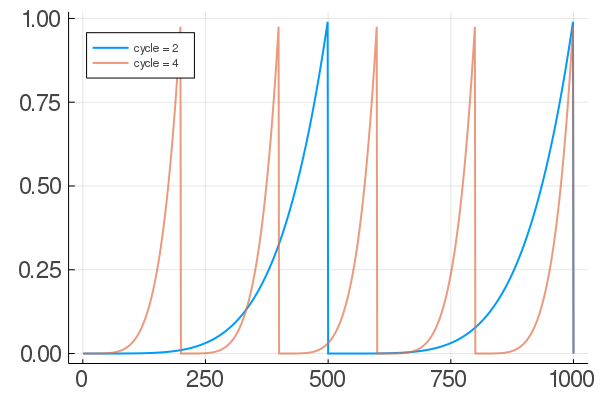
\includegraphics[width=\textwidth]{figures/Asched_c.png}}
    \caption{(a)\label{fig:aschedc}}
\end{subfigure}
\hfill
\centering
\begin{subfigure}[b]{0.48\textwidth}
    \scalebox{1}{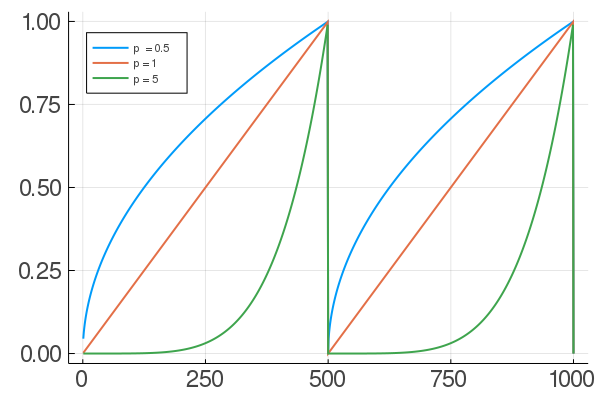
\includegraphics[width=\textwidth]{figures/Asched_p.png}}
    \caption{(b)\label{fig:aschedp}}
\end{subfigure}

\caption{Annealing schedules. \cref{fig:aschedc} shows two annealing schedules with $2$ cycles and $4$ cycles respectively. \cref{fig:aschedp} shows annealing schedules across $p  = 0.5, 1, 5$.}
\label{fig:acsched}
\end{figure}




\captionsetup[subfigure]{labelformat=empty}
\begin{figure}[t!]
    \centering 
\begin{subfigure}[b]{.48\textwidth} 
    \scalebox{1}{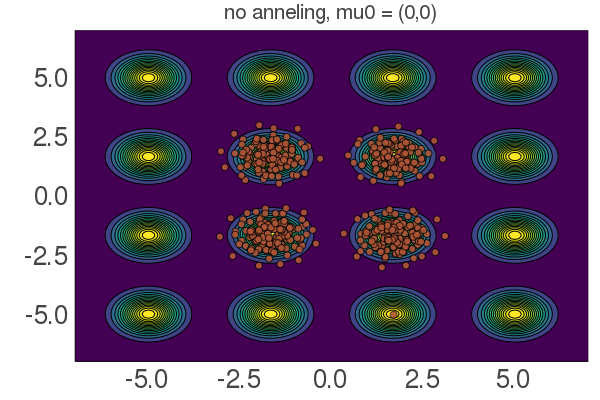
\includegraphics[width=\textwidth]{figures/T0_rms.png}}
    \caption{(a)\label{fig:T0_rms}}
\end{subfigure}
\hfill
\centering
\begin{subfigure}[b]{0.48\textwidth}
    \scalebox{1}{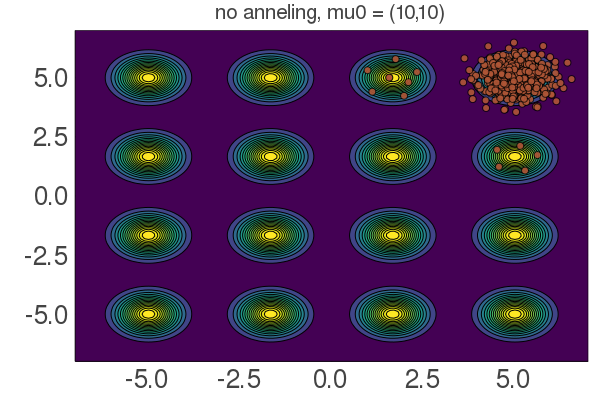
\includegraphics[width=\textwidth]{figures/T10_rms.png}}
    \caption{(b)\label{fig:T10_rms}}
\end{subfigure}
\hfill
\centering
\begin{subfigure}[b]{.48\textwidth} 
    \scalebox{1}{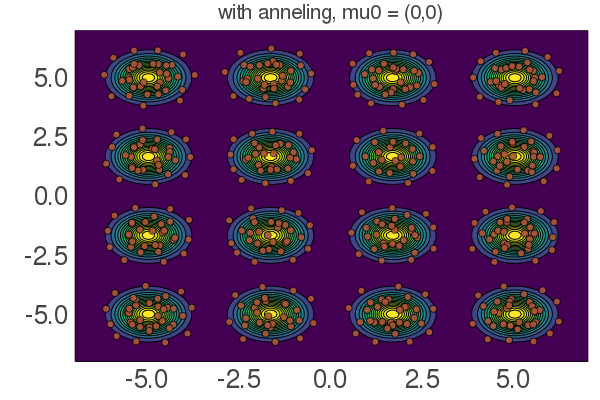
\includegraphics[width=\textwidth]{figures/T0_rms_anneal.png}}
    \caption{(c)\label{fig:T0_rms_anneal}}
\end{subfigure}
\hfill
\centering
\begin{subfigure}[b]{0.48\textwidth}
    \scalebox{1}{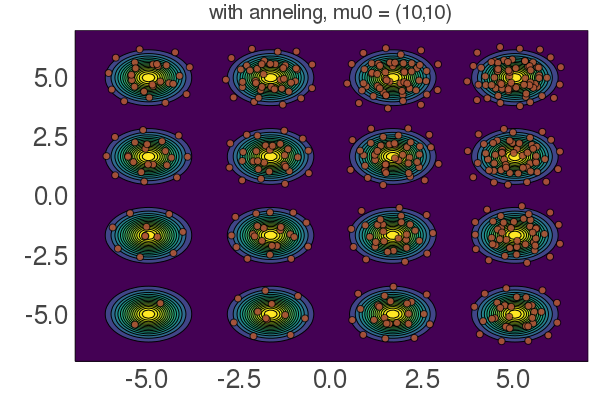
\includegraphics[width=\textwidth]{figures/T10_rms_anneal.png}}
    \caption{(d)\label{fig:T10_rms_anneal}}
\end{subfigure}
\caption{Comparison of SVGD (\cref{fig:T0_rms,fig:T10_rms}) and A-SVGD (\cref{fig:T0_rms_anneal,fig:T10_rms_anneal}) on the synthetic Gaussian mixture with 16 components with $\sigma = 0.5$ across two set of initial particles. }
\label{fig:SVGD_ASVGD}
\end{figure}


\subsection{Limitations of SVGD} 

A key limitation of SVGD is its
computational burden. Note that the deterministic updates described in \cref{eq:svgd} require the
evaluation of the kernel matrix and its gradient, which costs $\mcO(n^2)$.
This makes SVGD less practical compared to other particle sampling methods
such as sequential Monte Carlo sampler---which costs $\mcO(n)$---if we aim to
obtain a large number of samples from the target distribution.

The computation problem also occurs when calculating the gradient $\nabla \log
p(x)$ for all particles; this is particularly expensive in a large dataset
setting. Considering the target distribution as the posterior distribution
of a Bayesian model, i.e., $p(\theta) \propto \pi_0(\theta)\prod_{i = 1}^{m}
p(x_i \mid \theta)$ where $\pi_0$ denotes the prior distribution of $\theta$,
computing $\nabla \log p(\theta)$ exactly is not practical as $m$ is large.
Stochastic gradient estimates using subsampled data points can be applied in this case to make SVGD scalable.


In the following sections, we focus on another common issue of SVGD when the target
distribution $p(x)$ has multiple modes: the mixing problem, where the
particles collapse at a particular mode of the target distribution and fail
to distribute the particles to other high density regions. This is also known
as the \emph{mode collapse} phenomenon \citep{zhuo2018message,d2021annealed}
and appears often when the modes are distant from each other. The problem of
mode collapsing tends to be more severe in high-dimensional settings, but can
also be observed on a simple 2D Gaussian mixture target. Variants of SVGD are developed to resolve this issue (or at least alleviate the problem). 
For example, \citet{d2021annealed} adopts the tempering method from the MCMC literature \citep{zhang2019cyclical} that includes an annealing schedule in the SVGD updates; 
\citet{zhuo2018message} leverages the latent structure of the statistical model and converts the inference problem into a lower-dimensional space. 

In the next section,
we provide a clear illustration of the mixing issue on two synthetic examples
and introduce the annealed Stein variational gradient descent (A-SVGD), which tends to reduce the mixing issue. 
Further, we identify a central problem regarding the kernel bandwidth, which inspires our idea in \cref{sec:bw}.





\section{Annealed Stein variational gradient descent}\label{sec:asvgd} 




% \captionsetup[subfigure]{labelformat=empty}
% \begin{figure}[t!]
%     \centering 
% \begin{subfigure}[b]{.48\textwidth} 
%     \scalebox{1}{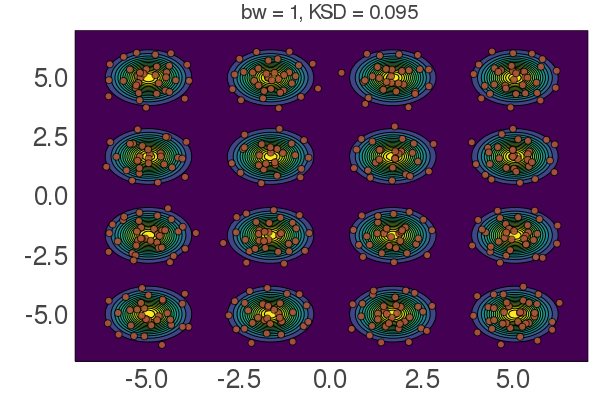
\includegraphics[width=\textwidth]{figures/bw1.png}}
%     \caption{(a)\label{fig:bw1}}
% \end{subfigure}
% \hfill
% \centering
% \begin{subfigure}[b]{0.48\textwidth}
%     \scalebox{1}{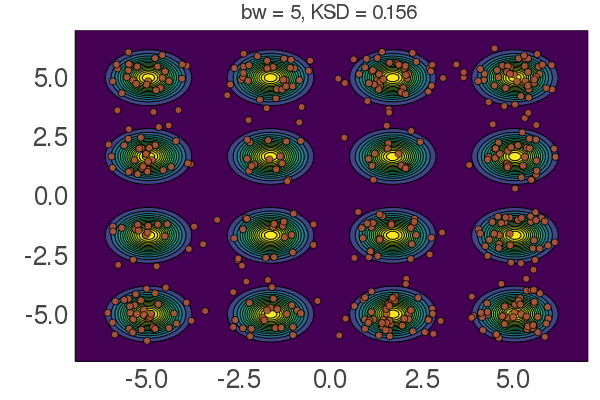
\includegraphics[width=\textwidth]{figures/bw5.png}}
%     \caption{(b)\label{fig:bw5}}
% \end{subfigure}
% \hfill
% \centering
% \begin{subfigure}[b]{0.48\textwidth}
%     \scalebox{1}{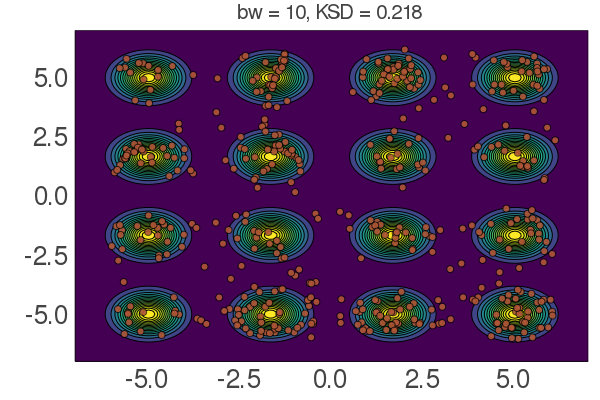
\includegraphics[width=\textwidth]{figures/bw10.png}}
%     \caption{(c)\label{fig:bw10}}
% \end{subfigure}
% \hfill
% \centering
% \begin{subfigure}[b]{0.48\textwidth}
%     \scalebox{1}{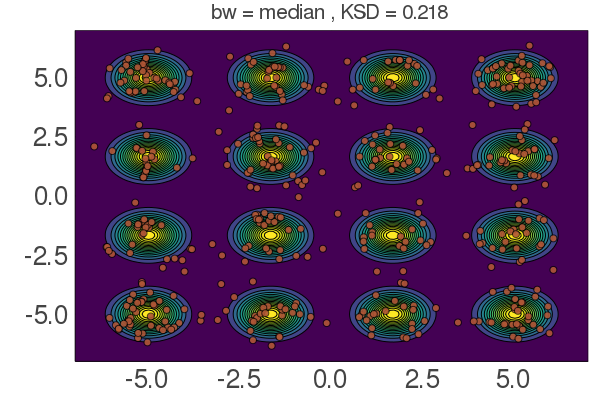
\includegraphics[width=\textwidth]{figures/bwmed.png}}
%     \caption{(d)\label{fig:bwmed}}
% \end{subfigure}

% \caption{Comparison of A-SVGD on the synthetic Gaussian mixture with 16 components across different bandwidth. }
% \label{fig:BW}
% \end{figure}








\captionsetup[subfigure]{labelformat=empty}
\begin{figure}[t!]
    \centering 
\begin{subfigure}[b]{.48\textwidth} 
    \scalebox{1}{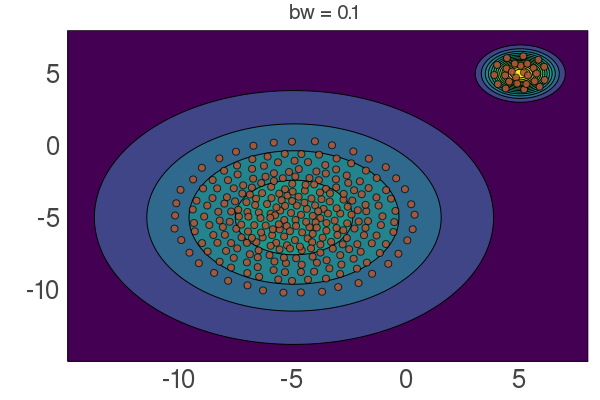
\includegraphics[width=\textwidth]{figures/bwsmall.png}}
    \caption{(a)\label{fig:bwsmall}}
\end{subfigure}
\hfill
\centering
\begin{subfigure}[b]{0.48\textwidth}
    \scalebox{1}{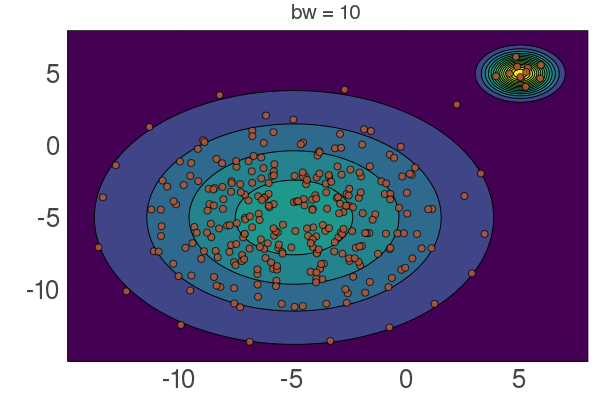
\includegraphics[width=\textwidth]{figures/bwlarge.png}}
    \caption{(b)\label{fig:bwlarge}}
\end{subfigure}
\hfill
\centering
\begin{subfigure}[b]{0.48\textwidth}
    \scalebox{1}{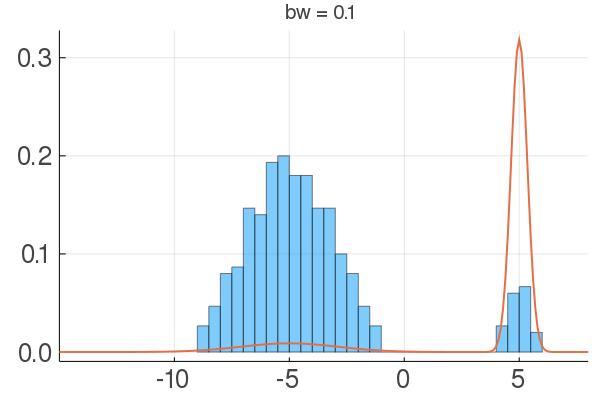
\includegraphics[width=\textwidth]{figures/slice_small.png}}
    \caption{(c)\label{fig:slice_small}}
\end{subfigure}
\hfill
\centering
\begin{subfigure}[b]{0.48\textwidth}
    \scalebox{1}{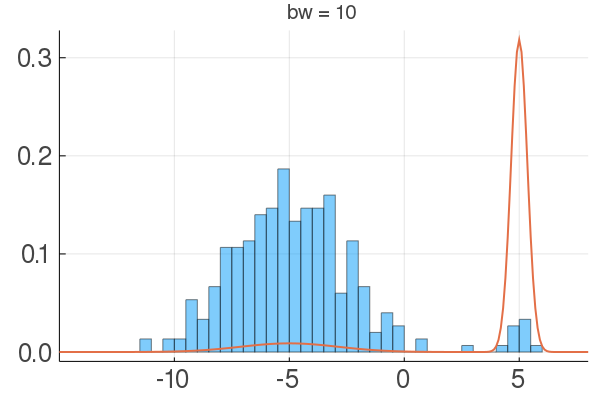
\includegraphics[width=\textwidth]{figures/slice_large.png}}
    \caption{(d)\label{fig:slice_large}}
\end{subfigure}


\caption{Comparison of A-SVGD on a 2-component Gaussian mixture with different bandwidth. \cref{fig:bwsmall,fig:bwlarge} show scatter plots of particles at the last iteration. \cref{fig:slice_small,fig:slice_large} show histograms of the particles by projecting the locations to the line $y = x$, where the orange curve denotes the density of Gaussian mixture along the slice $y = x$.}
\label{fig:differentBW}
\end{figure}


\begin{figure}[t!]
    
\end{figure}


\captionsetup[subfigure]{labelformat=empty}
\begin{figure}[t!]
    \centering 
\begin{subfigure}[b]{.48\textwidth} 
    \scalebox{1}{\includegraphics[width=\textwidth]{figures/mixGauss.png}}
    \caption{(a) \label{fig:bwlocal}}
\end{subfigure}
\hfill
\centering
\begin{subfigure}[b]{0.48\textwidth}
    \scalebox{1}{\includegraphics[width=\textwidth]{figures/slice_gauss.png}}
    \caption{(b)\label{fig:slicelocal}}
\end{subfigure}

\caption{A-SVGD with adaptive local bandwidth on a 2-component Gaussian mixture.}
\label{fig:localbw}
\end{figure}


\captionsetup[subfigure]{labelformat=empty}
\begin{figure}[t!]
    \centering 
\begin{subfigure}[b]{.48\textwidth} 
    \scalebox{1}{\includegraphics[width=\textwidth]{figures/grid_gs.png}}
    \caption{(a) $\{x_i^{(0)}\}_{i = 1}^{500} \distiid \distNorm(0\ind, 0.25I)$  \label{fig:bwlocal}}
\end{subfigure}
\hfill
\centering
\begin{subfigure}[b]{0.48\textwidth}
    \scalebox{1}{\includegraphics[width=\textwidth]{figures/grid_gs10.png}}
    \caption{(b) $\{x_i^{(0)}\}_{i = 1}^{500} \distiid \distNorm(10\ind, 0.25I)$ \label{fig:slicelocal}}
\end{subfigure}

\caption{A-SVGD with adaptive local bandwidth on a $4 \times 4$ Gaussian mixture.}
\label{fig:gridlocal}
\end{figure}



In this section, we provide a brief introduction of the annealed SVGD (A-SVGD), which is developed to address the mixing issue \citep{d2021annealed}, and use a few synthetic examples to identify a key limitation of the current work. The design of the synthetic example aims to  understand the influence of the kernel bandwidth on the behaviour of SVGD or A-SVGD and help us to build the intuition of picking a proper value. All the experiments performed in this report use the RMSprop update rule \cref{eq:rms}. We run both SVGD and A-SVGD with standard RBF kernel for $1000$ iterations under a constant learning rate $\gamma_k = 0.1$. 



We start with the development of A-SVGD. Considering the updates \cref{eq:svgd}, the optimal descent direction $ \hat{\phi}^{\star}(x)$ for the particle $x$ includes two parts: the driving force that moves the particle to a high density region of $p(x)$, and a repulsion that prevents the particles collapsing together. The specific derivation is as follows,
\[
    \hat{\phi}_k^{\star}(x)=\frac{1}{n} \sum_{j=1}^{n}\left[\underbrace{\kappa\left(x_{j}^{(k)}, x\right) \nabla \log p\left(x_{j}^{(k)}\right)}_{\text {driving force }}+\underbrace{\nabla_{x_{j}^{(k)}} \kappa\left(x_{j}^{(k)}, x\right)}_{\text {repulsion }}\right].
\]
When mode collapse occurs, particles produced by SVGD are trapped at some region and fail to explore the full support of $p(x)$. This often happens when the driving force dominates the repulsion. An intuitive solution is to boost the repulsion or scale down the driving force to enable a wider spread of the particles. 
\citet{d2021annealed} follows this intuition and modify the descent direction by introducing an annealing term $\alpha(k) \in [0, 1]$:
\[\label{eq:asvgd}
    \hat{\phi}_{\alpha_k}\left(x\right) = \frac{1}{n} \sum_{j=1}^{n}\left[ \alpha(k)\kappa\left(x_{j}^{(k)}, x\right) \nabla \log p\left(x_{j}^{(k)}\right)+ \nabla_{x_{j}^{(k)}} \kappa\left(x_{j}^{(k)}, x\right)\right].
\]
In particular, the authors suggest using a cyclical annealing schedule, i.e., 
\[
    \alpha(k)=\left(\frac{\bmod (k, K / C)}{K / C}\right)^{p},
\]
where $K$ is the total number of iterations, $C$ is the number of cycles, and $p > 0$ is an exponent factor that controls the speed of the transition between two phases. As demonstrated in \cref{fig:acsched}, smaller $p$ corresponds to a shorter period of the exploratory phase.  In all our experiments using A-SVGD, we set $ p = 1$ and $C = 2$. {\color{red} add a few sentence about cyclical }

Now we compare the performance of A-SVGD and SVGD on a synthetic Gaussian mixture (\cref{fig:SVGD_ASVGD}). The target distribution is a 2D mixture of $16$ Gaussian component with means equally distributed on a $4 \times 4$ grid with identical covariance $0.25I$.  We consider two different initialization particles: \cref{fig:T0_rms,fig:T0_rms_anneal} are initialized with $500$ \iid samples from $\distNorm(0, 0.25I)$; \cref{fig:T10_rms,fig:T10_rms_anneal} are initialized with $500$ \iid samples from $\distNorm(10, 0.25I)$. In this example, we use RBF kernel with $h = 0.5$. Note that in both initialization schemes, A-SVGD is able to explore all the modes 
while all the particles produced by SVGD collapse at the components close by the initialization. Comparing \cref{fig:T0_rms_anneal,fig:T10_rms_anneal}, one may notice that the performance of A-SVGD still depend on the location of the initial particles. 

% Although the A-SVGD manages to obtain a better mixing, its performance relies heavily on a good choice of kernel bandwidth. \cref{fig:BW} present the results of A-SVGD on the same target across $4$ different kernel bandwidth: $h = 1, 5, 10$ and the median heuristic described in \cref{sec:kernelchoice}. The initial particles are $500$ \iid samples from $\distNorm(0, 0.25I)$. We find that as $h$ increases (not even a large amount), the convergence of A-SVGD gets ruined. Moreover, the median trick suggested by \citet{liu2016stein} completely fails. For quantitative characterization of the sample qualities, we compute the kernelized Stein discrepancy,which shows a decreasing sample quality as $h$ increases. The key reason is that as the annealing schedule enables the points to traverse over different modes in the exploratory phase, the particles need to quickly converge to  the high-density region around them in the converging phase. As we mentioned previously, the driving force will push the samples along the $\nabla \log p(x)$. However, the driving force is a weighted summation of $\nabla \log p(x_i), i=1, 2, \dots, n$ and weights are controlled by the kernel. Adopting a large bandwidth tends to include misleading information from the particles that converge to other modes. 


% Even though the previous example prefers a smaller bandwidth, it does not mean that we should start with a small $h$.
In this experiment, we create a pathological yet simple example such that neither small nor large bandwidth is satisfying.  
Considering a two-component Gaussian mixture:
\[
\frac{1}{2}\distNorm\left( -5 \ind, 9I \right)  + \frac{1}{2}\distNorm\left( 5\ind, 0.25I \right).
\]
\cref{fig:differentBW} display the results of A-SVGD with $300$ initial particles sampled from $\distNorm(0\ind, 25I )$ using different kernel bandwidth $h = 0.1, 10$. With small $h$ particles located in the wide Gaussian component are overly contracted; with large $h$, almost all particles converges to the wide mode.
This is essentially due to the fact that the curvature of the local basin of two gaussian components is quite different. When using a wide kernel bandwidth, the driving force of those particles around the narrow Gaussian component is significantly influenced by gradient information $\log p(x)$ of the particles that are far away. As most particles are trapped in the wider Gaussian component, the driving force tends to point to the wide mode. Also, a large bandwidth leads to a stronger repulsion, which encourages the spread of particles. On the contrary, with small bandwidth---as shown in \cref{fig:bwsmall,fig:slice_small}---although the peaky Gaussian absorbs more particles, due to a weak repulsion introduced by the small bandwidth value,  particles at the wider Gaussian component are not spread enough, resulting in an underestimation of the variance. 
This hints at an important fact that using a universal kernel bandwidth for all particles is not ideal, and we should use different kernel bandwidths when updating each of the particles depending on its local basin of $\nabla \log p(x)$. In the next section, we propose an adaptive local bandwidth selection scheme that requires no input from the user. 




\section{A-SVGD with adaptive localized kernel} \label{sec:bw}
With the intuition obtained in the last section, we suggest using different bandwidth values for each particle and updates the bandwidth adaptively across the iteration.
The goal of this section is to design an adaptive procedure that learns a proper kernel bandwidth for each particle automatically.    
As illustrated in  \cref{fig:differentBW}, a careful choice of kernel bandwidth is necessary when the target distribution has multiple modes and one might consider using different bandwidth values at a different location.  Intuitively, a proper choice of the bandwidth should reflect the local geometry of   $\log p(x)$---the curvature of $\log p(x)$---which includes information of the Hessian $\nabla^2 \log p(x)$.  

We consider the anisotropical Gaussian kernel with covariance $\Sigma$,
\[
\kappa(x, x'; \Sigma) = \exp(-(x - x')^T \Sigma^{-1}(x- x')  ).  
\]
For computational reason, we propose to set $\Sigma $ to the absolute value of $\diag \left(\nabla^2 \log p(x) \right)$.


\bnprop
theoreticl justification for gaussian target
\enprop


Based on the empirical findings in \cref{sec:asvgd}, we find narrower mode requires smaller bandwidth while wider mode prefers a larger kernel bandwidth. 
Therefore, when updating $x_i$, an ideal choice of $h$ would be $1/ \sigma_1(\nabla^2 \log p(x_i))$, where $\sigma_1(M)$ denotes the maximal singular value of matrix $M$. However, solving  $\sigma_1(\nabla^2 \log p(x_i))$ is generally too expensive. We then use the maximal diagonal element of $\nabla^2 \log p(x_i)$ as approximation. The complete procedure of A-SVGD using adaptive local bandwidth is described in \cref{alg:ASVGD_bw}.

With other settings fixed, we apply \cref{alg:ASVGD_bw} to the previous two synthetic examples. As demonstrated in \cref{fig:localbw}, by using the local bandwidth, the samples in the wide component correctly characterize its variance and there is a certain amount of samples concentrate at the peak mode. This combines the advantages of both small $h$ and large $h$. And for the 16-component Gaussian example, since all Gaussian component shares the same covariance, we do not expect  A-SVGD with adaptive local bandwidth could outperform the previous results significantly. As shown in \cref{fig:gridlocal}, the result is quite similar to the A-SVGD using hand-tuned bandwidth; but importantly this  requires no user input in terms of kernel bandwidth.

It is worth pointing out that leveraging the Hessian of $\log p(x)$ introduces additional computation complexity. Evaluating the Hessian for all particles costs $\mcO(d^2N)$, denoting a quadratic growth as $d$ increases. This makes SVGD less practical in a high dimensional setting. In that case, we might consider using Gauss-Newton approximation to the Hessian matrix or other methods that approximate the second-order derivative using first-order information.
Also, when $n$ is large, evaluating $\nabla^2 \log p(x)$ for all the particles is impossible. But employing  stochastic estimates of the exact Hessian matrix is a reasonable approach.  








\section{Experiment} \label{sec:expt}




\subsection{logistic}



\subsection{GMM}



\subsection{Computation time}
% \section{Discussion} \label{sec:discuss}
some open problems: post hoc evaluation of the mixing issue. 

is there optimal annealing schedule.

is there any geometric interpretation of bandwidth

the computation effciency really depends on how fast computing the Hessian, maybe we can use Gauss-Newton approximation? using the outerproduct of grad




%%%%%%%%%%%%%%%%%%%%%%%%%%%%%%%%%%%%%%%%%%%%%%%%%%%%%%%%%%%%%%%%%%%%%%%%%
%% Reference
%%%%%%%%%%%%%%%%%%%%%%%%%%%%%%%%%%%%%%%%%%%%%%%%%%%%%%%%%%%%%%%%%%%%%%%%%%
\newpage
\bibliographystyle{apalike}
\bibliography{sources}


%%%%%%%%%%%%%%%%%%%%%%%%%%%%%%%%%%%%%%%%%%%%%%%%%%%%%%%%%%%%%%%%%%%%%%%%%
%% Appendix
%%%%%%%%%%%%%%%%%%%%%%%%%%%%%%%%%%%%%%%%%%%%%%%%%%%%%%%%%%%%%%%%%%%%%%%%%%
\newpage
\appendix
    % \section{Local bandwidth of two synthetic example}


    % \captionsetup[subfigure]{labelformat=empty}
    % \begin{figure}[H]
    %     \centering 
    % \begin{subfigure}[b]{.48\textwidth} 
    %     \scalebox{1}{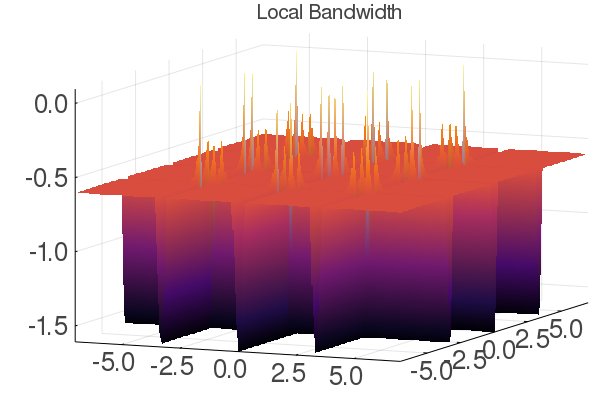
\includegraphics[width=\textwidth]{figures/bwsurf_grid.png}}
    %     \caption{(a)\label{fig:surf_grid}}
    % \end{subfigure}
    % \hfill
    % \centering
    % \begin{subfigure}[b]{0.48\textwidth}
    %     \scalebox{1}{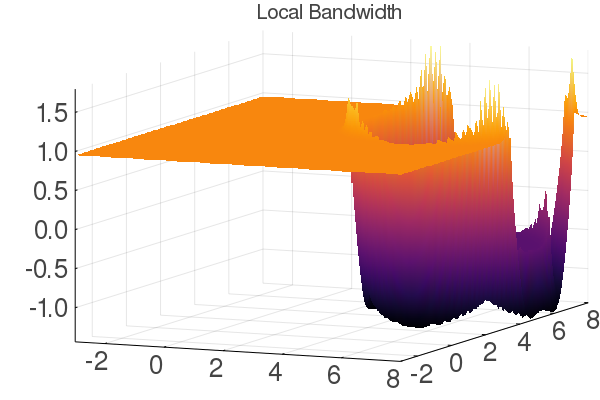
\includegraphics[width=\textwidth]{figures/bwsurf_mix.png}}
    %     \caption{(b)\label{fig:surf_mix}}
    % \end{subfigure}

    % \caption{Local bandwidth value for $4\times 4$ Gaussian grid (\cref{fig:surf_grid}) and 2-component Gaussian mixture (\cref{fig:surf_mix}).}
    % \label{fig:bwsurface}
    % \end{figure}



\section{Algorithms}

\begin{algorithm}[H] 
    \caption{SVGD} \label{alg:SVGD} 
\begin{algorithmic}
   \Procedure{SVGD}{$\{x_i^{(0)}  \}_{i = 1}^n$, $\nabla \log p(x)$, $\kappa(\cdot, \cdot)$,$\gamma_k$} 
   \For{ $k=0, 1, \dots, K-1$}
        \For{$i = 1, 2, \dots, n$}
        \State $x_{i}^{(k+1)} \leftarrow x_{i}^{(k)}+ \gamma_k \hat{\phi}_k^{\star}\left(x_{i}^{(k)}\right)$ where $\hat{\phi}_k^{\star}(\cdot)$ is defined in \cref{eq:svgd}
        \EndFor
    \EndFor
    \State \Return $\left\{x_i^{(K)}  \right\}_{i = 1}^n$ 
   \EndProcedure 
\end{algorithmic}
\end{algorithm}

\begin{algorithm}[H] 
    \caption{A-SVGD with local bandwidth} \label{alg:ASVGD_bw} 
\begin{algorithmic}
   \Procedure{SVGD}{$\{x_i^{(0)}  \}_{i = 1}^n$, $\nabla \log p(x)$, $\nabla^2 \log p(x)$,$\gamma_k$, $\alpha(t)$} 
   \For{ $k=0, 1, \dots, K-1$}
        \For{$i = 1, 2, \dots, n$}
        \State $\Sigma_i \gets 1/(\max \left\{\diag \nabla^2 \log p\left( x_{i}^{(k)}\right) \right\}$
        \State $\kappa(x, x'; \Sigma_i)\gets \exp(-(x - x')^T \Sigma_i^{-1}(x- x')  )$
        \State $x_{i}^{(k+1)} \leftarrow x_{i}^{(k)}+ \gamma_k \hat{\phi}_{\alpha_k}\left(x_{i}^{(k)}\right)$ where $\hat{\phi}_{\alpha_k}(\cdot)$ is defined in \cref{eq:asvgd}
        \EndFor
    \EndFor
    \State \Return $\left\{x_i^{(K)}  \right\}_{i = 1}^n$ 
   \EndProcedure 
\end{algorithmic}
\end{algorithm}










\end{document}
